% ----------------------------------------------------------
% Teste test1_3_e5b32class10_20231211_215013
% ----------------------------------------------------------
\subsubsection{Teste test1_3_e5b32class10_20231211_215013 - AlexNet (Is That a Santa)}

Informações utilizadas para o treinamento.

\begin{table}[ht]
   \centering
   \caption{Treinamento}
   \label{tab:modelos}
   \begin{tabular}{| c | c | }
      \hline 
      \textbf{Informação} & \textbf{Descrição} \\
      \hline \hline 
      Rede & AlexNet \\
      \hline
      Número de épocas & 5\\
      \hline
      Tamanho do lote & 32\\
      \hline
      Taxa inicial & 0.01 \\
      \hline
      Taxa de decaimento & 0.0005 \\
      \hline
      Total de classes & 10\\
      \hline
      Dataset & CIFAR-10\\
      \hline
   \end{tabular} 
\end{table}

Resultados obtidos após treinamento.

\begin{tabular}{lrrrr}
\toprule
  Unnamed: 0 &  precision &  recall &  f1-score &    support \\
\midrule
    airplane &   0.744973 &  0.8150 &  0.778415 &  1000.0000 \\
  automobile &   0.928090 &  0.8260 &  0.874074 &  1000.0000 \\
        bird &   0.622936 &  0.6790 &  0.649761 &  1000.0000 \\
         cat &   0.580715 &  0.5360 &  0.557462 &  1000.0000 \\
        deer &   0.760042 &  0.7190 &  0.738952 &  1000.0000 \\
         dog &   0.771654 &  0.5880 &  0.667423 &  1000.0000 \\
        frog &   0.708502 &  0.8750 &  0.782998 &  1000.0000 \\
       horse &   0.868721 &  0.7610 &  0.811301 &  1000.0000 \\
        ship &   0.836795 &  0.8460 &  0.841372 &  1000.0000 \\
       truck &   0.762148 &  0.8940 &  0.822826 &  1000.0000 \\
    accuracy &   0.753900 &  0.7539 &  0.753900 &     0.7539 \\
   macro avg &   0.758458 &  0.7539 &  0.752458 & 10000.0000 \\
weighted avg &   0.758458 &  0.7539 &  0.752458 & 10000.0000 \\
\bottomrule
\end{tabular}


\begin{figure}[ht]
 \begin{center}
   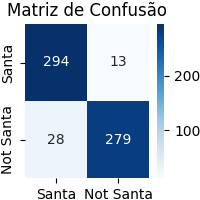
\includegraphics[scale=1]{tests/test1_3_e5b32class10_20231211_215013/confusion_matrix.png}
  \caption{Matriz de Confusão}
  \label{fig:fig03}
 \end{center}
\end{figure}

\begin{figure}[ht]
 \begin{center}
   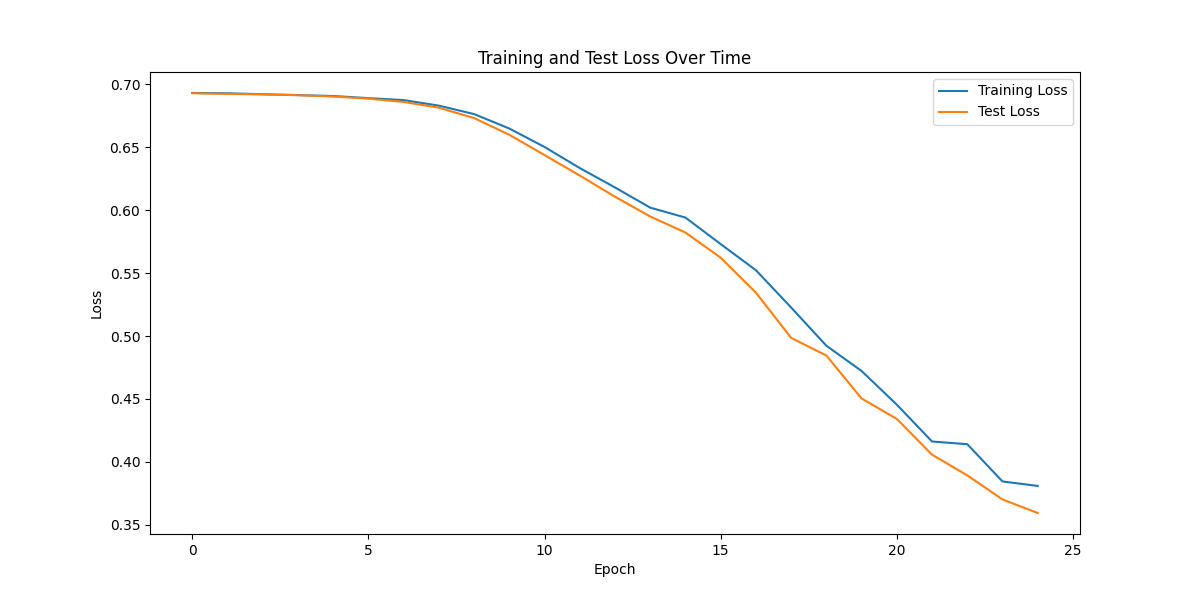
\includegraphics[scale=0.8]{tests/test1_3_e5b32class10_20231211_215013/loss_over_time.png}
  \caption{Gráfico de Perda}
  \label{fig:fig04}
 \end{center}
\end{figure}
